\documentclass[11pt,letterpaper]{article}

% Load some basic packages that are useful to have
% and that should be part of any LaTeX installation.
%
% be able to include figures
\usepackage{graphicx}
% get nice colors
\usepackage{xcolor}

% change default font to Palatino (looks nicer!)
\usepackage{apjfonts}
% load some useful math symbols/fonts
\usepackage{latexsym,amsfonts,amsmath,amssymb}

% comfort package to easily set margins
\usepackage[top=1in, bottom=1in, left=1in, right=1in]{geometry}

% control some spacings
%
% spacing after a paragraph
\setlength{\parskip}{.15cm}
% indentation at the top of a new paragraph
\setlength{\parindent}{0.0cm}


\begin{document}

\begin{center}
\Large
{\bf Ay190 -- Worksheet 9} \\
\large
Xiangcheng Ma \\
Date: \today
\end{center}

\section*{Linear System}
(1) Using {\tt np.loadtxt} to read $A$ and $\bf b$: \\
{\tt A=np.loadtxt("LSEi\_m.dat")} \\
{\tt b=np.loadtxt("LSEi\_bvec.dat")} \\

The size of these systems are 10, 100, 200, 1000 and 2000 from $i=1$ to $5$. Using {\tt SciPy} routine {\tt numpy.linalg.slogdet} to calculate the logarithmic of the determinant of $A$ to determine whether these systems are solvable. The result is all of them can be solved.

(2) I provide my own Gauss elimination routine {\tt gaussian.py}. Inside it, I add a few sentence in order to jump out the routine and claim an error if the systems is not solvable. The routine has been widly tested using a series of different $3\times3$ systems, including some of extreme cases. The solutions are solved as ``{\tt LSEi\_soln.dat}". The time consumption is listed in Table~\ref{tb} and plotted in Figure~\ref{fig}. In general, it follows an $O(N^3)$ complexity.

(3) I use {\tt scipy.linalg.lu\_solve} routine, which is based on $LU$ decomposition method. The time comsumption is listed in Table~\ref{tb} and plotted in Figure~\ref{fig} for a reference. This routine is much faster than Gaussian elimination. It looks like a complexity of $O(N^n)$ ($n<3$) for smaller $N$, while incease to $O(N^3)$ for large $N$. However, this may result from system flutuations and therefore needs more tests.
\begin{table}[h]
\centering
\begin{tabular}{ccccc}
\hline\hline
$t$ (days) & E & $x$ (AU) & $y$ (AU) & steps \\
\hline
\multicolumn{5}{c}{$e=0.0167$} \\
\hline
91.0 & 1.58209228899 & -0.0112957219731 & 0.999796755471 & 4 \\
182.0 & 3.13096420068 & -0.999943518526 & 0.0106267706437 & 2 \\
273.0 & 4.67948910053 & -0.0328939450239 & -0.99931946851 & 4 \\
\hline
\multicolumn{5}{c}{$e=0.99999$} \\
\hline
91.0 & 2.30664638749 & -0.671217514443 & 0.00331500920351 & 7 \\
182.0 & 3.13618964107 & -0.999985403763 & 2.41628286027e-05 & 3 \\
273.0 & 3.96364377765 & -0.680720102446 & -0.00327602643159 & 7 \\
\hline\hline
\end{tabular}
\label{table}
\caption{Kepler Motion}
\end{table}


\begin{figure}[th]
\centering
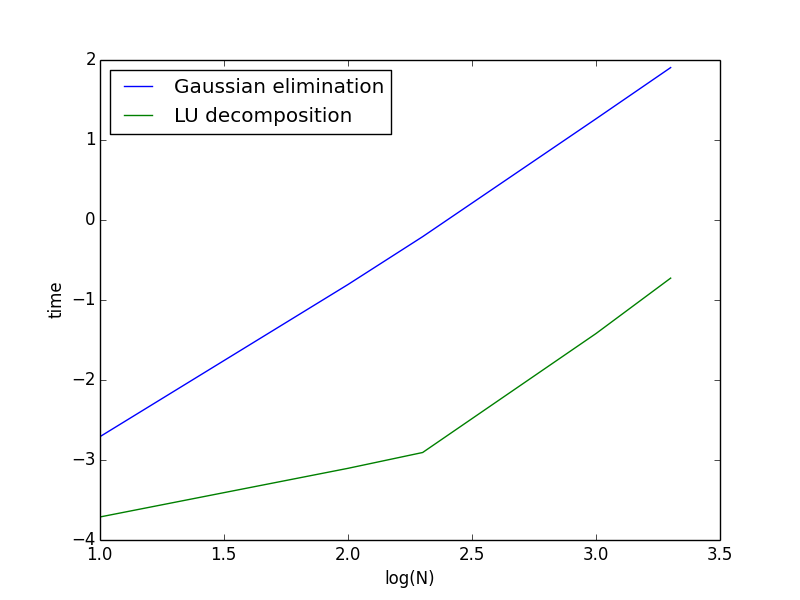
\includegraphics[width=1.0\textwidth]{fig.png}
\caption{Linear System Solver Time Consumption}
\label{fig}
\end{figure}



\end{document}
